%%%%%%%%%%%%%%%%%%%%%%%%%%%%%%%%%%%%%%%%%
% Large Colored Title Article
% LaTeX Template
% Version 1.1 (25/11/12)
%
% This tex file was produced using a template  downloaded from:
% http://www.LaTeXTemplates.com
% Original author:
% Frits Wenneker (http://www.howtotex.com)
% License:
% CC BY-NC-SA 3.0 (http://creativecommons.org/licenses/by-nc-sa/3.0/)
%
% All intellectual content presented in the article itself remains the sole work of the author.
%
%----------------------------------------------------------------------------------------
%	PACKAGES AND OTHER DOCUMENT CONFIGURATIONS
%----------------------------------------------------------------------------------------

\documentclass[DIV=calc, paper=a4, fontsize=11pt, twocolumn]{scrartcl}	 % A4 paper and 11pt font size
\usepackage{lipsum} % Used for inserting dummy 'Lorem ipsum' text into the template
\usepackage[english]{babel} % English language/hyphenation
\usepackage[protrusion=true,expansion=true]{microtype} % Better typography
\usepackage{amsmath,amsfonts,amsthm} % Math packages
\usepackage[svgnames]{xcolor} % Enabling colors by their 'svgnames'
\usepackage[hang, small,labelfont=bf,up,textfont=it,up]{caption} % Custom captions under/above floats in tables or figures
\usepackage{booktabs} % Horizontal rules in tables
\usepackage{fix-cm}	 % Custom font sizes - used for the initial letter in the document
\usepackage{hyperref}
\usepackage[format=hang]{caption}
\usepackage{caption}


%====== added by BO 08.07.2016 ========================
\usepackage{tcolorbox}
\usepackage{enumitem}
%====== edits by BO from 08.07.2016 down to here ===========

\usepackage{sectsty} % Enables custom section titles
\allsectionsfont{\usefont{OT1}{phv}{b}{n}} % Change the font of all section commands

\usepackage{fancyhdr} % Needed to define custom headers/footers
\pagestyle{fancy} % Enables the custom headers/footers
\usepackage{lastpage} % Used to determine the number of pages in the document (for "Page X of Total")

% Headers - all currently empty
\lhead{}
\chead{}
\rhead{}
% Footers
\lfoot{}
\cfoot{}

% PAGE NUMBERING:
\rfoot{\footnotesize Page \thepage\ of \pageref{LastPage}} % "Page 1 of 2"

\renewcommand{\headrulewidth}{0.0pt} % No header rule
\renewcommand{\footrulewidth}{0.4pt} % Thin footer rule

\usepackage{lettrine} % Package to accentuate the first letter of the text
\newcommand{\initial}[1]{ % Defines the command and style for the first letter
\lettrine[lines=3,lhang=0.3,nindent=0em]{
\color{DarkGoldenrod}
{\textsf{#1}}}{}}

%----------------------------------------------------------------------------------------
%	TITLE SECTION
%----------------------------------------------------------------------------------------

\usepackage{titling} % Allows custom title configuration
\newcommand{\HorRule}{\color{DarkGoldenrod} \rule{\linewidth}{1pt}} % Defines the gold horizontal rule around the title
\pretitle{\vspace{-30pt} \begin{flushleft} \HorRule \fontsize{25}{25} \usefont{OT1}{phv}{b}{n} \color{DarkRed} \selectfont} % Horizontal rule before the title
\title{Counting Everyone: A Model for Electoral Reform in Canada} % Your article title
\posttitle{\par\end{flushleft}\vskip 0.5em} % Whitespace under the title
\preauthor{\begin{flushleft}\large \lineskip 0.5em \usefont{OT1}{phv}{b}{sl} \color{DarkRed}} % Author font configuration
%\author{Brendan Osberg} % Your name
\author{Author name redacted (Peer-review submission copy)} % Your name

\postauthor{\footnotesize \usefont{OT1}{phv}{m}{sl} \color{Black} % Configuration for the institution name
% Your institution

\par\end{flushleft}\HorRule} % Horizontal rule after the title
\date{} % Add a date here if you would like one to appear underneath the title block


%----------------------------------------------------------------------------------------
\begin{document}
%\maketitle % Print the title
\thispagestyle{fancy} % Enabling the custom headers/footers for the first page


% Keywords: Electoral reform, proportional representation, voting, Quotient, mixed-member.
% Color for online-only is sufficient. Print version figures can be black&white

%%----------------------------------------------------------------------------------------
%% SUMMARY SECTION

% Latest word count (10.05.2020): 4,100
\section*{Summary}
\renewcommand{\thefigure}{S-\arabic{figure}}

The parsimonious mixed member (PMM) model is a voting system designed such that:

\begin{itemize}
\item Every constituency is represented by a specific MP, and every vote counts. 
\item Proportional seating ensures that no party is underrepresented, relative to its popular support. 
\item Parties have greater incentive to win local races than in traditional mixed-member (MM).
\item Spoiled, and minor-party ballots are not misattributed to major parties (as is tacitly done in traditional MM).
\item Changes to the current system are minimized and have evidence of success in an existing democracy.
\end{itemize}

To illustrate, projected results from the 2015 election are converted to quotients (see supplement) shown in Fig.~\ref{fig:sumQParties-2015-338-cutoff}, along with an example threshold defining a proportional legislature with 338 members. 
\begin{figure}[h!]
  \includegraphics[width=0.50\textwidth,clip]{Figs/Qparties_2015_338_cutoff}
%\captionsetup{labelformat=empty}
  \caption{Projection of `quotients' (see main text, supplement) from the 2015 Canadian federal election, for each party. The grey transparent line provides a threshold for the largest 338 quotients (above the cutoff) to be converted into seats for a proportional legislature. Ridings are incorporated in Fig.~\ref{fig:sumQParties-2015-ordered}. }
\label{fig:sumQParties-2015-338-cutoff}
\end{figure}

Fig.~\ref{fig:sumQParties-2015-ordered} accounts for the local winners of each constituency while allocating additional seats for proportionality, similar to the additional member system (AMS), but with the minimum possible number of additional seats.

\begin{figure}[h!]
\includegraphics[width=0.50\textwidth,clip]{Figs/QParties_2015_ordered}
\caption{ In PMM, we rank quotients from all parties, giving priority to constituency seats (to the left), similar to AMS. The lowest-quotient from this group defines the threshold (horizontal, grey) for supplementary seats (right of the `jump' in this data). Parliament is then proportional with all ridings accounted for, and quotients below this threshold are ignored.}
\label{fig:sumQParties-2015-ordered}
\end{figure}

Finally, Fig.~\ref{fig:hypo_2015_sum} projects the change in standings in parliament with PMM. Further details and examples are provided in the main text.

\begin{figure}[h!]
  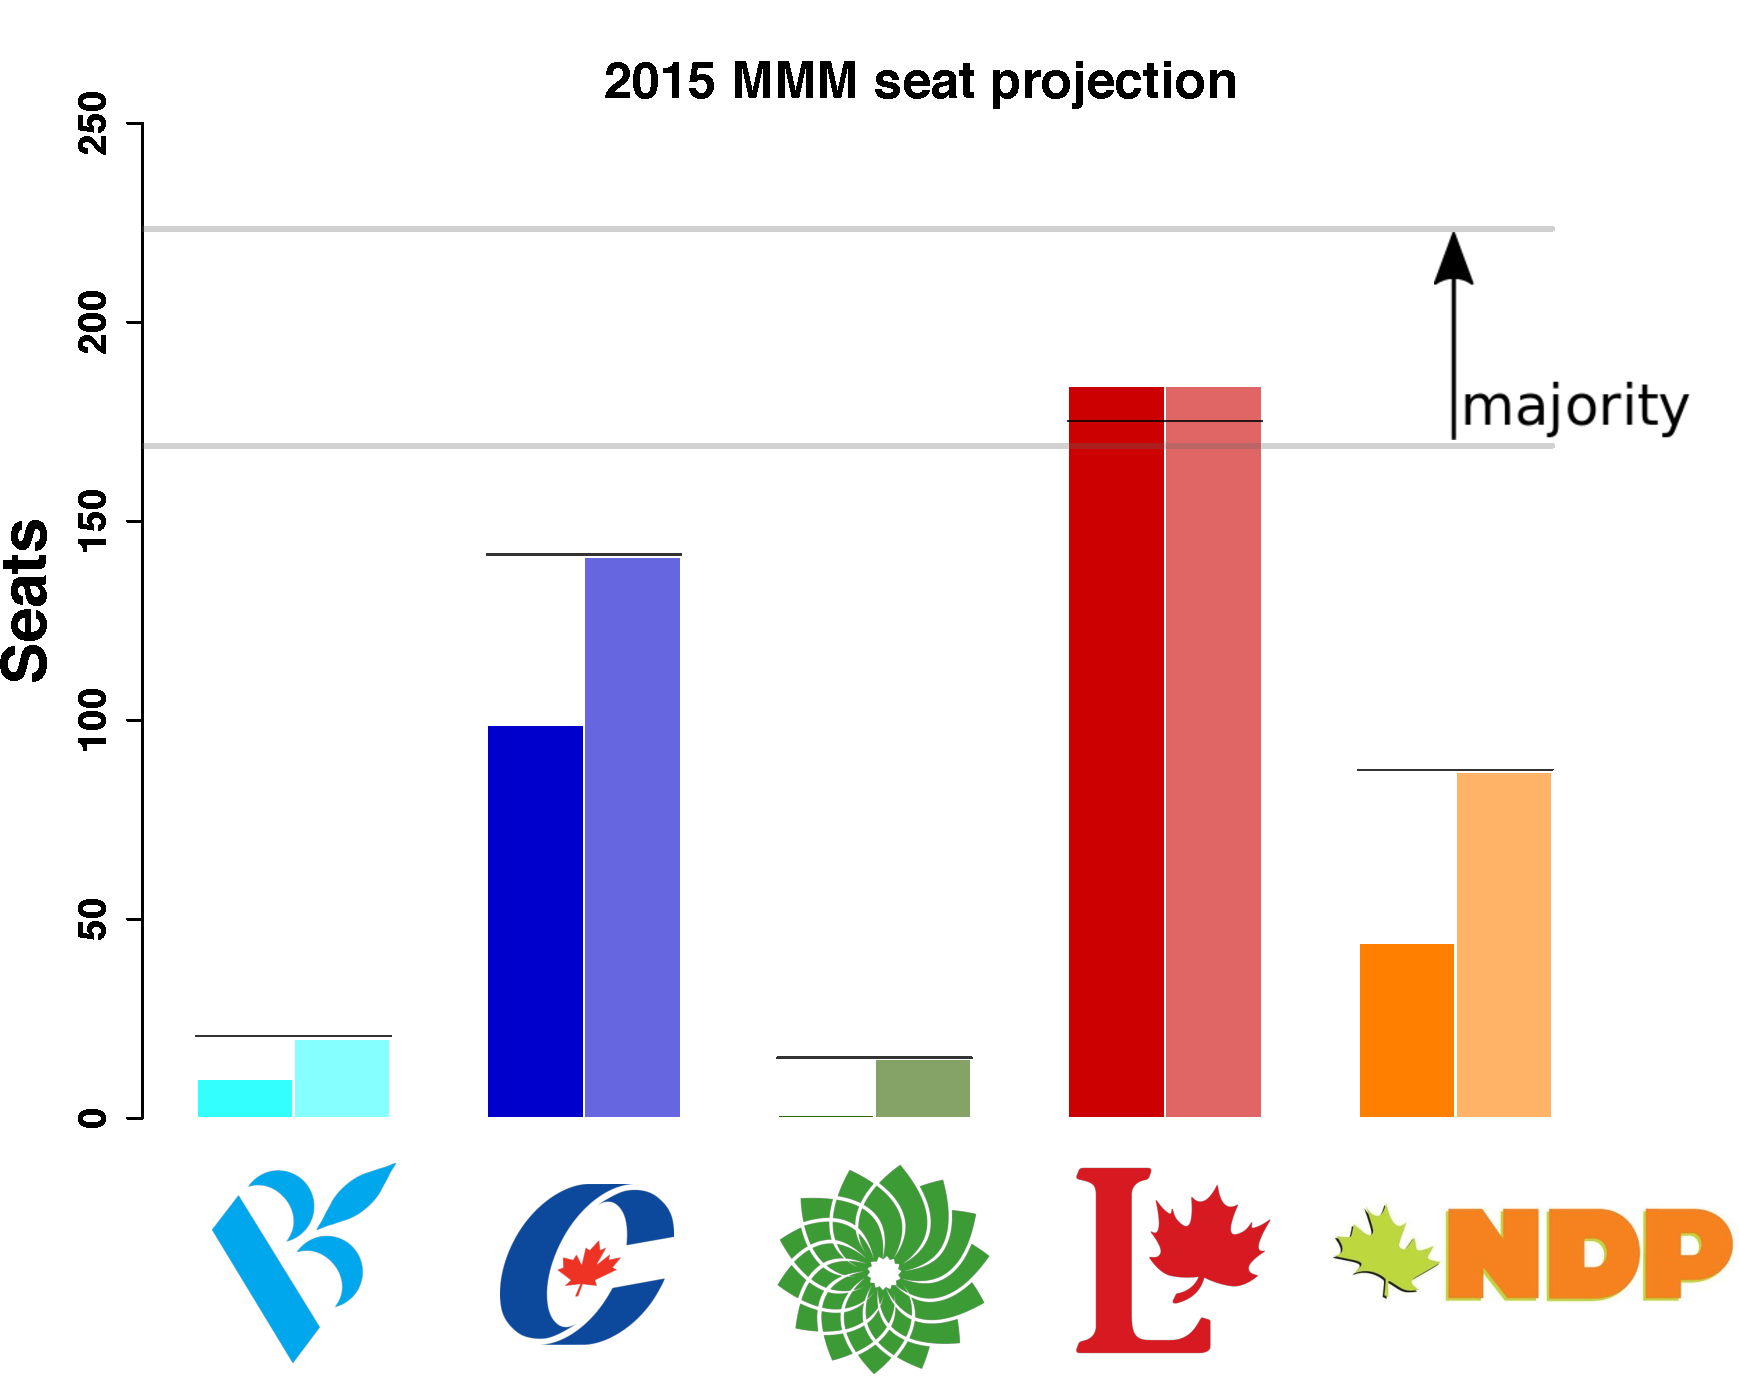
\includegraphics[width=0.50\textwidth,clip]{Figs/2015_seat_projection}
  \caption{Projected seat distribution following the 2015 federal election, using actual results (left) alongside projected results of this model from the same electorate in transparency (right). The bar defining majority control is shown in grey transparency for both cases, while a finer black line for each party shows the number of seats that would correspond to their share of the popular vote.}
\label{fig:hypo_2015_sum}
\end{figure}

\pagebreak

%%----------------------------------------------------------------------------------------
%	   BEGINNING MAIN ARTICLE: ABSTRACT
 
\maketitle % Print the title
\thispagestyle{fancy} % Enabling the custom headers/footers for the first page

\renewcommand\thefigure{\arabic{figure}}
\setcounter{figure}{0}
%  \setcounter{page}{-3}

% The first character should be within \initial{}
%----------------------------------------------------------------------------------------
%	Abstract
%----------------------------------------------------------------------------------------
\begin{abstract}
\textbf{\underline{Abstract:}}
Recent calls for Canada’s current first-past-the-post (FPP) system to be reformed have generally avoided the thorny details of precisely \emph{which} changes ought to be made. 
The ‘parsimonious mixed-member’ (PMM) model, described here, is inspired by the mixed-member (MM) proportional representation (PR) system currently used in, for example, Germany, but is ‘parsimonious’ in that the number of MPs brought into parliament to reach proportionality is minimized.
Like traditional MM, PMM preserves individual relationships between voter and MPs, and eliminates under-representation. However, it improves on MM by preserving the incentive for parties to win local races, avoids unnecessary ‘dilution’ of constituency representatives, and avoids misattribution of spoiled ballots to major parties, by preserving voters’ rights to vote for \emph{no party}. 
PMM is also conservative -it modifies our existing FPP system with the minimal changes necessary to resolve its most obvious problems, without creating new ones. PMM fixes only what is broken. 
\end{abstract}


%----------------------------------------------------------------------------------------
%	BEGIN ARTICLE
%----------------------------------------------------------------------------------------
\section{Background and Motivation}
\label{sec:BM}

Assessing the performance of any electoral system requires first clarifying what it is intended to achieve.
While referenda establish unambiguous levels of support for options `yes' and `no', general elections involve various overlapping preferences that are impossible to disentangle with a single ballot mark.
The mechanics of Canada's FPP system suggest that the question posed to voters during elections is as follows:
%--- make a textbox here.
\begin{tcolorbox}[colback=white!5!white,colframe=blue!55!black]
{\textbf{Q1:} } `Which local candidate do you wish to represent your riding?'
\end{tcolorbox}
In practice, however, there are clearly many other considerations on voters' minds.
Such considerations might include: `Which national party do you support?', or `Which national leader do you wish to be prime minister?', or `Which viable local candidate(s) might you be \emph{satisfied} with?' (particularly relevant for `strategic'\footnote{A `strategic'  consideration is defined here as one based on the anticipation of other voters' behaviour.} voters).

In the current system, each riding's member of parliament (MP) is selected so as to maximize the number of voters whose {\textbf{Q1}} preference is satisfied, while all others are simply discarded. Governments are then formed based on which party has the most MPs.
In translating popular will to electoral mandate, there is clearly information loss in this process.

While it is unclear what priority voters attach to each of the above questions during elections, historically, \textbf{Q1} may have better described the formation of government when geography and limited communications left ridings more isolated.
Advances in telecommunications, for example, have since made national politics more widely accessible.

% REMOVED: Moreover, voters are now influenced by sophisticated statistical pre-election polling. This has increased the importance of `strategic' factors in both a formal\cite{Leadnow_environics} and informal sense.
% The distinction between the `ideal' and the `satisfactory' choice is particularly hard to quantify \--and contentious;
% Whether or not voters \emph{should} `vote with their hearts' within the current system is a value judgement that will not be addressed here.
%The simple fact is that many voters \emph{do} feel pressured to vote strategically.


More importantly, under the modern FPP system, citizens of nearly every political persuasion have at some point felt underrepresented \--albeit at different times. It is unlikely that the `joy' of being \emph{over-}represented in certain periods offsets the frustration of under-representation later, and
 national unity can hardly be aided by such stark divisions and periodic resentment, even if a kind of de facto proportionality is established on long-term averages.

% REMOVED: Perhaps what can be said at the moment is that various political parties have now had their `turn' to take advantage of the undemocratic peculiarities of our current system and that the time is now ripe to end these disparities and make our system democratic at all times.


The benefits of changing such systems can be seen in studies that `clearly identify' higher voter turnout rates in voting systems with some form of PR\cite{Blais_1990}
 across many nations. In a particularly relevant case study, New Zealand was found to have succeeded in `fostering more positive attitudes about the efficacy of voting' \cite{NZ_PR_results}.

There are some risks, however. It was shown in Germany that some systems of PR can have unintended consequences when it was inconveniently revealed that their PR system allowed \emph{negative} vote weights in some rare circumstances\cite{Die_Zeit_negative_vote}
%\footnote
% {
% The German system allocated overhang seats (i.e. constituency seats won in excess of popular share) to each state independently, while popular vote share was calculated across the entire country.
% In certain situations, a party could win seats that would have been assigned to them anyway (via overhang constituency seats), with little change to its share of the national vote; effectively eliminating their `overhang'. A seat in the Bundestag reserved for proportionality might then be shifted elsewhere, resulting in a net loss of one seat for the party.
% This problem arises partly because of the fixed number of seats in the parliament, and the need for each seat to be assigned to \emph{someone}. This quandary prompts the question: if a seat is not necessary to represent a constituency, nor to establish proportionality, then why not eliminate it entirely? We will return to this question in Sec.~\ref{sec:model_proposal}.
% }.
This pathological case led to the system being ruled unconstitutional before the formula was corrected.
Clearly, it is important to avoid such issues in a Canadian system, however this serves to highlight a potential peril.
Voting systems are complex, involving millions of participants, and the current system, while imperfect, has worked at least well enough to maintain our democracy for over a century.
The more tinkering that is done, the greater the potential for harm.
Indeed, while a recent Canadian poll\cite{Broadbent_poll} showed overwhelming support for at least some change to the political system, about half of respondents were wary of \emph{too much} change \--evidently preferring a system that has been tried and tested.
For these reasons, keeping change to a minimum while resolving specific problems in our existing system will be a principle theme in the following sections.


%------------------------------------------------------------------------------------------------
\section{Defining the Goal}
%------------------------------------------------------------------------------------------------
\label{sec:goal_list}

Here, a list of desirable characteristics in an electoral system are enumerated to serve as guiding principles of the model that will be proposed in Sec.~\ref{sec:model_proposal}.
\begin{enumerate}
\item \textbf{Accountability} must be maintained between all citizens and an MP whose role is to represent \emph{them} specifically. Without this, governments become impersonal and estranged.
\item \textbf{Every vote must count} productively. Scenarios in which citizens are discouraged from voting by thinking that their vote will not matter (or, much worse, that it might actively work against their interests) must be precluded.
\item \textbf{Proportionality} of national support for major groups \--either political parties, or national leaders\-- must be reasonably approximated.\footnote{
An \emph{exact} mirror of popular support would generally require as many MPs as voters, which is clearly impractical. Rounding, at a minimum, is necessary.
}
\item   \textbf{Simplicity.} The ballot must be sufficiently easy to understand to avoid any widespread difficulty in filling it out.

\item  \textbf{The significance of local races should be preserved}. Parties should have an incentive to run credible candidates in each riding, and these direct representatives should control as much of parliament as possible.
\item \textbf{Conservatism.} While imperfect, our current democratic system has many advantages (and already fulfils items 1, 4 and 5 above). We should change our existing system only as much as is necessary to satisfy the remaining objectives, and no more. Changes that \emph{are} proposed to our existing system should have some evidence of success in an existing democracy.
\end{enumerate}

%----------------------------------------------------------------------------------------
%	DIFFERENT PROPOSALS FOR REFORM
%----------------------------------------------------------------------------------------

\section{Prospective Models}
\label{sec:alt_models}

With the list in Sec.~\ref{sec:goal_list}, we can consider some of the current electoral systems elsewhere in the world and how well they meet our criteria. For example, the \emph{list system}, as used in Israel, produces party representation in proportion to the popular vote; it is easily understood, and it ensures that every vote counts \---satisfying requirements 2, 3, and 4.
The ranking of the party lists, however, is generally determined within the party, leaving candidates no signal as to their individual popularity in any particular riding. Moreover, without separate electoral districts, the connection of voters to a specific MP is eliminated. 
For a geographically concentrated country, perhaps this is not so great a problem, but for Canada there are sure to be many regions, far-removed from Ottawa where citizens feel estranged by system that offers them no clear answer to the question `who speaks for me?'. Similar criticisms have been made by scholars as Enid Lakeman\cite{Lakeman}.

The single transferable vote (STV) \---as used in Ireland, for example\cite{Irish_howto_vote_doc}
\--- allows voters to  rank their preferences and if a voter's first choice fails to be elected (or receives such support that additional votes would be superfluous), their vote is transferred to the voter's second preference in a constituency, and so on.
Satisfying requirement 1 above would require maintaining single-seat constituencies, making STV equivalent to a ranked ballot (RB). The system would then satisfy requirements 1, 4, 5, (and arguably 6).
% REMOVED: Although the Irish balloting process involves some increased complexity in the \emph{counting} process, from each voter's perspective, the concept of ranked preference is easily understood and can be made without the need for strategizing.

This, however, is \emph{not} a form of PR.
Rather than allocate fair proportions of seats to voters' \emph{ideal} choice, RBs explicitly incorporates voters' willingness to compromise into their ballot, and maximizes the number of voters with a \emph{satisfactory} representative.
Altering our voting system in this way would be akin to supplementing question \textbf{(Q1)} from Sec.~\ref{sec:BM} above with the following:

\begin{tcolorbox}[colback=white!5!white,colframe=blue!55!black]
`\ldots and if your ideal candidate cannot be elected, whom \emph{then}?'.
\end{tcolorbox}

Part of the appeal of RBs is conservatism \--it is merely a matter of gathering additional information from the voters for possible contingencies, and no structural changes to parliament are required. Candidates can also review their tally of votes to ascertain the enthusiasm of their supporters, and the degree of overlap with other candidates.

It has been argued\cite{Record} that RBs would benefit the currently governing Liberal party, as `centrist' parties are more likely to accumulate second-place votes than parties on either end of the political spectrum.
Whether such an advantage would be fair or not (i.e., should we consider only voters' pure beliefs, or also their willingness to compromise?) is a value judgment that will not be addressed here. Rather, does such an advantage exist at all?

While the precise rate of strategic voting remains unclear, voters who currently vote for mainstream candidates may be more likely to support an underdog if they know that their vote has a kind of `insurance policy' in place.
A sufficient shift in first-choice ballots from these risk-averse voters may result in surprise upsets with currently centrist seats being won by other parties who were superficially thought to have no chance of winning.
Given the uncertainty in the influence of strategic considerations, it remains  unclear which political party will benefit most from ranked preferences.

This latter consideration, however, underscores a problem with RBs:  there is no obvious mechanism for filtering out small parties to prevent parliament from becoming fragmented. As such, RBs could lead to the proliferation of many small parties
(unlike both the list system and  mixed-member models which generally impose a minimum threshold in popular support for proportional seating of `major' parties).
Moreover, the RB system also falls short of our criteria in two important ways.
First: not all votes will `count' in this system.
Suppose a voter lives in a riding where a single candidate has such overwhelming support as to virtually guarantee victory; or the voter only feels comfortable giving their support to one or two candidates, none of whom have a chance of winning.
In either of these cases, the rationale to stay home and not bother voting is weakened (compared to FPP) but not eliminated entirely.

Secondly, this system still will not ensure proportionality: RBs, like FPP ballots, allow for scenarios in which a single party receives widespread support across the country, and yet still insufficient support in any particular ridings to be awarded many seats. 
Such a party will at least have a better \emph{chance} of winning local races, compared to FPP, but the core problem of disparity between the cumulative national popular vote, and parliamentary representation is not fully resolved with RBs.

That being said, criticism of RBs should not be overstated here; there is no criteria by which the RB system performs \emph{worse} than the current FPP, and several areas where it would provide significant improvement.
In the following, however, we will explore models that provide even greater improvement.


% --------  German MM ----------------
\subsection{The Mixed-Member Solution}
\label{sec:german_model}

The mixed-member (MM) model is another common alternative, a well-known example of which is seen in Germany.

Today German citizens are presented with two votes: the first ballot selects a representative for their constituency, and these representatives fill up half of the Bundestag.
The second ballot is used to establish proportionality between the parties using candidates from a party list established prior to the vote
(for clarity, we will refer to the former as `constituent' MPs  and the latter as `supplementary' MPs).
To prevent government paralysis through the proliferation of many small parties, a party must win more than 5\% of the popular vote to be entitled to any supplementary seats.
%\footnote{
%When PR was first introduced in Germany after the first world war in the form of the list system it produced a string of unstable successive governments and extremist parties. After the second world war, the founders of the German government, anxious to avoid the mistakes of their predecessors, added this clause limiting additional seat allocation only to parties above a threshold of support.
%}.

There are many subtle benefits this system could offer Canada.
First, this form of PR maintains the individual connection of every voter with a single MP who is accountable to their constituency.
Second, every vote counts; even if a voter is in a region that's already a lock for an opposing candidate, they may still express their support for their preferred party, leading to large-scale proportionality.
% \--in practice, one might argue that the influence of parties on national politics is of greater prominence than any individual candidate, and many German political parties place greater emphasis on the second ballot in rallying get-out-the-vote campaigns.
Moreover, the twin ballots of this system allow voters to distinguish their vote between local candidates and their parties.
Constituent MPs can then gauge their mandate: an MP who wins a seat in a riding where their party did poorly on the second ballot can claim to have been elected on individual merits rather than party label (and perhaps take some liberty in voting their conscience in the legislature). Conversely, an MP who narrowly won in a strong riding for their party should feel greater pressure to toe the party line.
%------------------------------------------=====
Finally, as with RB, while the counting may have some additional complexity, the voting is simple enough for all to understand, requiring only an additional mark \--which provides additional information. Traditional MM satisfies requirements 1, 2, 3, and 4 from Sec.~\ref{sec:goal_list}.

However, what if a voter wishes to support \emph{only} their local candidate, and no party? Since traditional MM fills up available seats by priority of major parties, each major party's share of seats is determined by its proportion of \emph{votes among major parties}, not among votes overall. As such, there is a (relatively small) share of the population whose share of seats is misattributed to a party for whom they expressed no support (see Supplement Sec.~\ref{sec:outliers} for more details.)

Moreover, once in the elected body, supplementary MPs are equal in number to constituent MPs, and occupy half of the Bundestag.
The voting power of constituent MPs is then significantly reduced, and voters who rely on their representative to act on their behalf may feel less empowered.

This begs the question: is it really necessary to \emph{double} the size of parliament? Doing so in Canada would represent a rather drastic change to the system, and would dilute the mandate of constituent MPs significantly.
There are other democracies with smaller fractions of their elected body assigned to supplemental MPs, and yet they too are fixed in size.
To phrase the question more generally: `How many supplementary MPs are \emph{needed} to satisfy proportionality?'
\emph{This} question has a mathematically unambiguous answer for any given election that will be shown in the following section.
If indeed the purpose of supplementary MPs is to establish proportionality, then any MPs beyond this are superfluous \--and detrimental to constituent-based representation.

%----------------------------------------------------------------------------------------
%   MY PROPOSAL
%----------------------------------------------------------------------------------------
\section{Parsimonious Mixed-Member}
\label{sec:model_proposal}

Consider a hypothetical election under MM with three parties: $X$, $Y$, and $Z$. Suppose that after comparing each party's share of constituency seats to its share of the popular vote, party $X$ is underrepresented in parliament, party $Y$ is represented appropriately, while party $Z$ is over-represented.

A standard algorithm for allocating seats proportionally is the D'Hondt method, which relies on defining a series of Quotients for each party $m$:
\begin{equation}
\label{eq:Qdefn}
Q_{m,j} = \frac{V_m}{j}.
\end{equation}

Here, $V_m$ is the total number of votes given to party $m$, and $j$ is the list index (see Supplement).
Thus, the quotients enumerate party $m$'s vote total divided into halves, and then thirds, quarters, \ldots etc. The utility of these quotients is that a single threshold on these values can be used to define a proportional body; a graphical illustration is shown in Fig.~\ref{fig:Qlist_byparty_2019}.


% \begin{figure}[h!]
\begin{figure} % the h! forces the figure to be "here", not necessary.
  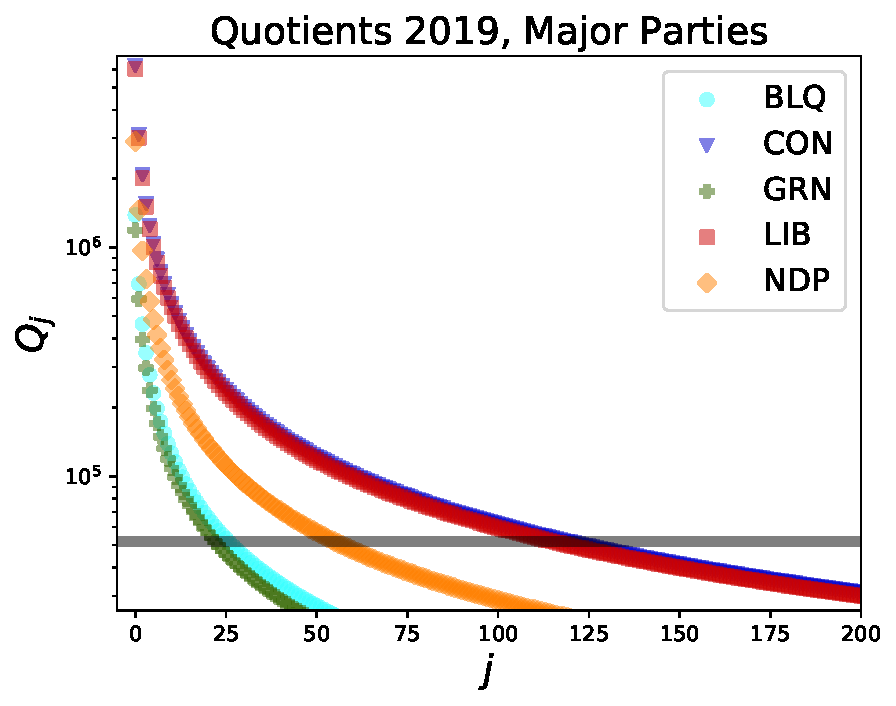
\includegraphics[width=0.50\textwidth,clip]{PR_calcs/data/raw_2019/PMM_out/PMM_Qlist_byparty}
  \captionsetup{format=default}
  \caption{Quotient projections (using Eq.~\ref{eq:Qdefn}) from the 2019 Canadian federal election, for each party. A proportional legislature can be defined by drawing a horizontal line anywhere on this graph, separating quotients that are awarded seats (above) from ones that are discarded (below). The grey transparent line, for example, separates the largest 338 quotient values and could, in principle, determine a proportional legislature. Ridings are addressed in the following Fig.~\ref{fig:Qlist_all_2019}. }
\label{fig:Qlist_byparty_2019}
\end{figure}

The above method provides a natural prioritization for seat allocation.
The party with the largest quotient not yet assigned to a seat, at any given time, is the most underrepresented (relative to its popular support), and has priority claim to the next seat assignment, should one be available.
It is for this reason that the mixed-member systems in Wales and Scotland are referred to as Additional Member Systems (AMS).
% REMOVED: \--the D'Hondt quotients determine the next `additional member' to the legislative body.

With this system, in our hypothetical scenario, party $X$ will be the first in line to receive additional seats. As seats are assigned, and parliament grows, at some point, party $Y$ will begin to receive seats as well, since its relative share of parliament is decreasing.
Towards the end of this process, seats are assigned to parties $X$, $Y$, \emph{and} $Z$ in an uneven rotation, with each addition counteracting the effects of the previous. The original need for supplementary seats (i.e., proportionality) has been satisfied, but the process continues until all empty seats of the fixed-size assembly are filled.

This is where parsimonious mixed-member (PMM) departs from existing MM/AMS systems, by adding supplementary seats only until proportionality is established. To illustrate this graphically, we can re-order the list of quotients from Eq.~\ref{eq:Qdefn} for all parties by magnitude, but giving priority to seats that were already assigned by constituency races, as in Fig.~\ref{fig:Qlist_all_2019}.
\begin{figure}
  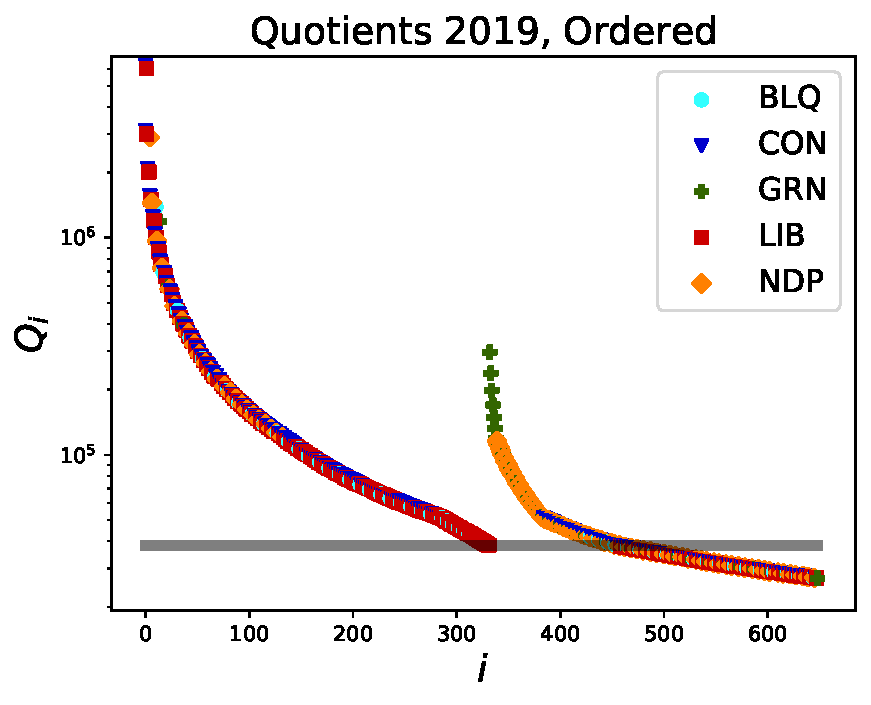
\includegraphics[width=0.50\textwidth,clip]{PR_calcs/data/raw_2019/PMM_out/PMM_Qlist_all}
  \captionsetup{format=default}
  \caption{ In PMM, we order all the quotients from Fig.~\ref{fig:Qlist_byparty_2019} into two groups, giving priority to constituency seats (to the left). The lowest-quotient from this group then defines the lower limit for parties to be granted supplementary seats (to the right of the `jump' in the data). Any quotient below this threshold can be ignored }
\label{fig:Qlist_all_2019}
\end{figure}
Here, the smallest quotient associated with a constituency seat defines a threshold for supplementary seats. By assigning supplementary seats only until this point, we ensure that proportionality is established with the minimum possible number of supplementary seats.

While this method can ensure that no party is under-represented, parties that were \emph{over-}represented, based on FPP results, can retain a small degree of that advantage, since there is generally a small fraction of votes that cannot be assigned to any major party. These ballots default towards the prior FPP results by inhibiting the addition of \emph{any} supplemental MPs.
This is another difference from many other MM systems, where the significance of the first ballot is eclipsed by the second. In PMM, the first ballot still matters, and voters can choose `no party' (see Supplement Sec.~\ref{sec:outliers} for more details).

As to \emph{who} should fill these supplemental seats for each party, this can be decided on by a number of criteria.
In the German case, Strattmann notes\cite{Stratmann}, ``The ranking on the list is determined, in part, by the party members' prominence, seniority, interest group approval of the nomination, and evidence of longstanding prior party activities".
For regional representation, most existing MM systems have a fixed parliament size, with a corresponding number of supplemental seats for each region of the country.

In PMM, the same broad representation can be achieved if each party's list of supplemental candidates is ranked, internally, according to a rotating scheme that distributes representation across the different regions and provinces of the country.
Explicitly regional parties \--such as the Bloc Quebecois, for example\-- might opt-out of such a formula, and draw only from a particular region.
Otherwise, giving parties an opportunity to introduce some MPs from regions where they normally win fewer seats may serve to partially erode sharp regional political divisions.

%----------------------------------------------------------------------------------------
%	WHAT WOULD OTHER ELECTIONS LOOK LIKE?
%----------------------------------------------------------------------------------------

\section{Projections Based on Previous Results}
\label{sec:projections}

It is impossible to say with certainty what results previous elections would have produced with this system, since historical voting data already contain the effects of strategic voting, low turnout from disaffected voters, and other influences. Changing the voting system will likely affect the behaviour of some voters.

Nevertheless, we can make approximate projections. Let us assume that in 2019, if this system had been in place, the same citizens would have shown up at their polling stations and that their regional (i.e., first) ballot would be unchanged.
Let us further assume that all voters' second ballot vote would go to the party of their preferred first-ballot candidate.
% \begin{figure}[h!]
\begin{figure}
  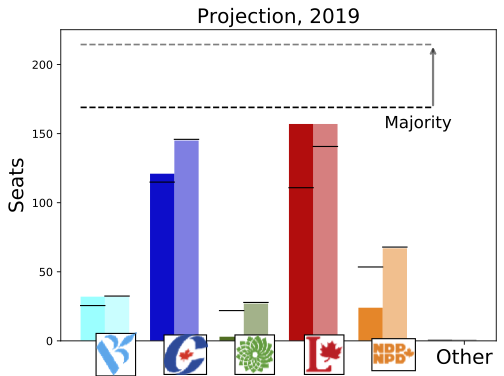
\includegraphics[width=0.50\textwidth,clip]{PR_calcs/data/raw_2019/PMM_out/PMM_projections}
  \caption{ Projected seat distribution following the 2011 federal election, using actual results (left) alongside projected results of this model from the same electorate in transparency (right). The bar defining majority control is shown in grey transparency for both cases, while a finer black line for each party shows the number of seats that would correspond to their share of the popular vote.
}
\label{fig:projection_2019}
\end{figure}
Under these assumptions, Fig.~\ref{fig:projection_2019} shows the breakdown of seats that was actually observed in 2019 alongside the total seat count that would be allotted to each party in the PMM system.
Likewise, Fig.~\ref{fig:projection_2011} shows the same calculation for the 2011 election (for the 2015 election, please see supplement).

\begin{figure}[h!]
%\begin{figure}
  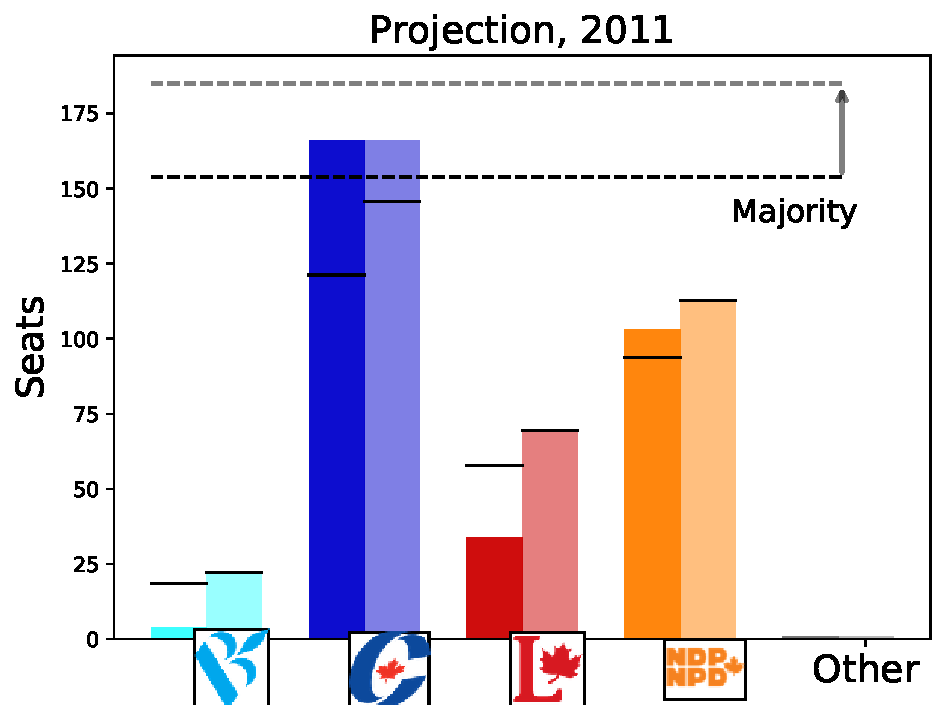
\includegraphics[width=0.50\textwidth,clip]{PR_calcs/data/raw_2011/PMM_out/PMM_projections}
  \caption{ Seat distribution following the 2011 federal election, using the same conventions as in Fig.~\ref{fig:projection_2019}.}
\label{fig:projection_2011}
\end{figure}

Note that in each case, while no party is underrepresented, only the initially over-represented party (Conservative in 2011, Liberal in 2015 and 2019) remains slightly over-represented (see Supplement).
As discussed in the previous section, this advantage serves to motivate parties to win constituency races.

There is nothing about this system that inherently prevents majority governments \--indeed, a party's lead could be \emph{increased} into a majority with the second-ballot results. However, in practice, most governments with some form of PR have shown a tendency towards coalitions. Germany, for example, has established coalition governments as the norm in recent decades.

%----------------------------------------------------------------------------------------
%	Discussion and Conclusion
%----------------------------------------------------------------------------------------
\section{Discussion and Conclusion}

While there is much discussion about the need for electoral reform in Canada, there remains a lack of detailed discussion as to what type of reforms should be made, and what their implications would be.
Making the right choice depends on defining the criteria for success, as Sec.~\ref{sec:goal_list} is intended to do.
The STV/ranked ballot satisfies enough of these criteria to merit serious consideration, and yet the mixed-member model comes even closer.
The latter can be further improved by limiting supplementary MPs to the minimum number necessary for proportionality, thus preserving the incentive for parties to win first-ballot races, and allowing voters the option to eschew party labels entirely.

%REMOVED: Under PMM, the share of supplementary MPs would never exceed what is already being practiced in a functioning democracy. That is to say, for a parliament with $N$ constituencies, the number of supplementary MPs is constrained from 0 (where the result would be identical to our current FPP system), up to a maximum of $N$ (which would reproduce the German system). In practice, the number of supplementary MPs is likely to be approximately $N/3$, as shown in Sec.~\ref{sec:projections}.
%
While MM has worked well in many countries, a known vulnerability to abuse exists via \emph{decoy} lists.
% REMOVED: as seen in the \emph{Scorporo} system during the 2001 Italian Chamber of Deputies election, for example.
Through this tactic, candidates run as ostensibly independent (or affiliated with an obscure `decoy' party) while in practice having the tacit support of a major party.
The party's supporters are then encouraged to cast split ballots and elect this de facto party member \emph{in addition to} a supplementary seat for the same party, perverting the compensatory intention of supplementary seats.

Various measures can, and have, been employed to prevent this \--direct exclusion under certain criteria being generally the most effective.
For example, 2nd ballots can be excluded if they are attached to a first ballot cast for a victorious independent candidate (this is, in fact, a major reason why the ballots are not separated in Germany.)
There are many other MM systems with effective restrictions to prevent decoy-list-tactics while still allowing good-faith voters to choose between both candidate and party. The problem is by no means insurmountable; nevertheless, it must be emphasized that it would be a grave mistake to overlook this problem entirely.

With that caveat in mind, PMM satisfies all of the requirements listed in Sec.~\ref{sec:goal_list}: A personal connection between every voter and a representative is maintained, citizens of all ridings will know that their vote will count towards the final result, and that their vote will not be misattributed to a larger party, should they support an independent candidate.
The ballots are simple and the end result of proportionality of parliamentary seats, based on popular vote, is intuitive.
Likewise, from the perspective of candidates, this two-bit communication, sends a clearer message to policy-makers as to what their constituents were actually voting for.
Once these representatives take office, their power is diluted as little as possible, while ensuring no party is underrepresented, and they will have been chosen from the best of their parties, as their parties still have incentive to win local races.
For all these reasons, Canada should adopt PMM.

\begin{thebibliography}{99}

\bibitem{Abramson_2010}
Abramson, P. R., Aldrich, J. H., Blais, A., Diamond, M., Diskin, A., Indridason, I. H., … Levine, R. (2010). Comparing Strategic Voting Under FPTP and PR. Comparative Political Studies, \textbf{43}(1), 61–90.
%https://doi.org/10.1177/0010414009341717

\bibitem{Banducci_Karp}
Banducci, S.A. and Karp, J.A. Perceptions of Fairness and Support for Proportional Representation.
\emph{Political Behavior} \textbf{21}, 217–238 (1999). https://doi.org/10.1023/A:1022083416605

\bibitem{Broadbent_poll}
David Coletto and Maciej Czop,
{\color{blue} \href{https://d3n8a8pro7vhmx.cloudfront.net/broadbent/pages/4770/attachments/original/1448994262/Canadian_Electoral_Reform_-_Report.pdf?1448994262}{Canadian Electoral Reform}},
{\emph{Public Opinion on Possible Alternatives} }, December 2015

\bibitem{Blais_1990}
Andre Blais and Kenneth Carty,
`Does Proportional Representation Foster Voter Turnout?'
European Journal of Political Research \textbf{18}(2):167-181, (1990)

\bibitem{Blais_2006}
Blais, Andr\'e and Bodet, Marc Andr\'e. . Does Proportional Representation Foster Closer Congruence Between Citizens and Policy Makers? Comparative Political Studies, \textbf{39}(10): 1243–1262 (2006)
% https://doi.org/10.1177/0010414005284374

\bibitem{Cox}
Cox, G. W. and Fiva, J. H. and Smith, D. M.  The Contraction Effect: How Proportional Representation Affects Mobilization and Turnout. The Journal of Politics, \textbf{78}(4), 1249–1263 (2016)
% doi:10.1086/686804

\bibitem{Fiva}
Fiva, J. and Hix, S. Electoral Reform and Strategic Coordination.
British Journal of Political Science, 1-10. (2020)
%doi:10.1017/S0007123419000747

\bibitem{Geys_2006}
Geys, Benny. 2006. “Explaining Voter Turnout: A Review of Aggregate-
level Research.” Electoral Studies \textbf{25}(4): 651.

\bibitem{Horowitz}
Horowitz, Donald L. "Electoral Systems: A Primer for Decision Makers."
Journal of Democracy \textbf{14}(4): 115-127 (2003).
%doi:10.1353/jod.2003.0078.

\bibitem{Karp_Banducci}
Jeffrey A. Karp and Susan A. Banducci
`The Impact of Proportional Representation on Turnout: Evidence from New Zealand.',
\emph{Australian Journal of Political Science}, \textbf{34}(3),363-377 (1999)

\bibitem{Lakeman}
E. Lakeman,
{ \emph{Power to Elect} }, Suffolk, U.K.: The Electoral Reform Society (1982) pp 59-63.

\bibitem{Leadnow_environics}
Environics,
{\color{blue} \href{http://www.votetogether.ca/pages/localpolling/}{`13 Swing Riding Polls - Wave One'}}, August 19, 2015

\bibitem{Leduc}
Leduc, L. The Failure of Electoral Reform Proposals in Canada. Political Science, \textbf{61}(2), 21–40. (2009)
%https://doi.org/10.1177/00323187090610020301

 \bibitem{Die_Zeit_negative_vote}
{\color{blue} \href{http://www.zeit.de/2005/39/Wahl\_paradox}{`Viele Farben, keine Wahl'}},
 { \emph{Die Zeit} }, September 22, 2005


%%%%%
\bibitem{Boston}
Boston, Jonathan and Church, Stephen and Bale, Tim, The Impact of Proportional Representation on Government Effectiveness: The New Zealand Experience,
Australian Journal of Public Administration,
\textbf{62}(4): 7-22 (2003)
%url = {https://onlinelibrary.wiley.com/doi/abs/10.1111/j..2003.00345.x},
%eprint = {https://onlinelibrary.wiley.com/doi/pdf/10.1111/j..2003.00345.x},
%abstract = {It is often claimed that proportional representation (PR) undermines government effectiveness, including decisional efficacy, fiscal prudence, electoral responsiveness and accountability. Drawing on New Zealand's experience since the introduction of a mixed-member proportional (MMP) electoral system in 1996, this article examines the impact of the new voting system on government effectiveness. Although government durability has been substantially reduced and the policy-making process has become more complex, governments under MMP appear to be no less able to address major policy problems or respond to changing economic circumstances. Moreover, New Zealand has maintained continuous fiscal surpluses under MMP — a radical departure from the protracted, and often large, deficits that characterised the previous two decades under a majoritarian electoral system.},
%doi:10.1111/j..2003.00345.x,
%%%%%


\bibitem{Record}
 Michael Taube
{\color{blue} \href{http://www.therecord.com/opinion-story/6692466-liberals-electoral-reform-would-stack-the-deck-in-their-favour/}{ \emph{Liberals electoral reform would stack the deck in their favour} } },
Waterloo Region Record, May 27, 2016

\bibitem{Selb}
 Selb, P. (2009). A Deeper Look at the Proportionality—Turnout Nexus. Comparative Political Studies,
 \textbf{42}(4), 527–548.
 %https://doi.org/10.1177/0010414008327427


\bibitem{Stratmann}
Thomas Strattman
{\color{blue} \href{https://www.researchgate.net/profile/Thomas_Stratmann2/publication/228978716_Party-Line_Voting_and_Committee_Assignments_in_the_German_Mixed_Member_System/links/0c96052d411ad2b0ae000000/Party-Line-Voting-and-Committee-Assignments-in-the-German-Mixed-Member-System.pdf}{Party-Line Voting and Committee Assignments in the German Mixed Member System}}
Department of Economics, George Mason University

\bibitem{Irish_howto_vote_doc}
Department of the Environment, Community and Local Government, Ireland
{\color{blue} \href{https://www.laois.ie/wp-content/uploads/Guide-to-Irelands-Electoral-System-2.pdf}{Guide to Ireland’s PR-STV Electoral System}}

\end{thebibliography}


%%----------------------------------------------------------------------------------------
%           SUPPLEMENT
 
\clearpage
\renewcommand{\theequation}{S.\arabic{equation}}
\renewcommand{\thesection}{S.\arabic{section}}
\setcounter{section}{0}
\setcounter{equation}{0}
% \setcounter{page}{1}
% \pagenumbering{roman}

%----------------------------------------------------------------------------------------
%	Supp
%----------------------------------------------------------------------------------------
\section*{Supplemental Material}

One challenge to creating proportionality in mixed-member (MM) systems is that there is no fair or practical way of \emph{removing} representatives from parties that are over-represented.
Seats can be added, however, and so the additional member system (AMS) is another common name that highlights how MPs are added to an existing body to approach proportionality.
Generally, the D'Hondt highest averages method is used for this process, which we briefly review now. None of the mathematical details presented here are necessary for the average voter to either (a) cast their ballot, or (b) appreciate the correspondence in proportionality between popular vote and final seat distribution.

Assume a parliamentary body must represent $N$ constituencies, after an election involving $M$ major parties. A `major' party is defined as any party whose popular support exceeds the 5\% threshold on the 2nd ballot\footnote{Minor parties are ignored, so unless otherwise stated, `major' is implied. Likewise, a vote for a `party' refers to the 2nd ballot.}.
The index  $m \in \left\{0, .., M-1\right\} $  refers to each of the $M$ parties specifically, and quotients $Q_{m,j}$ for each party $m$ are defined as

\begin{equation}
\label{eq:DhondtSupp}
Q_{m,j} = \frac{V_m}{j},
\end{equation}

where $j \in \left\{ 1,.., \infty \right\}$ is an index\footnote{Conventionally, this might be written as $j+1$ in the denominator, with initial value $j=0$; the above has been chosen with initial value $j=1$ for readability}, and  $V_m$ is the number of votes for party $m$, out of a total of $\hat{V}$. Let $V^I$ denote the sum of 2nd ballots that were either spoiled, or cast for minor parties that failed to meet the 5\% threshold, thus:
\begin{equation}
\label{eq:sum_Vm}
V^I + \sum_m V_m = \hat{V}.
\end{equation}
Let $C_m$ represent the number of direct constituent seats that party $m$ was awarded from the total $N$, and $C^I$ the number of seats won by independent candidates, or candidates from minor parties,
\begin{equation}
\label{eq:sum_Cm}
C^I + \sum_m C_m = N.
\end{equation}

In practice, $C_m$ and $V_m$ will clearly be correlated, since voters tend to prefer candidates and parties along similar ideological lines. However, since $C_m$ is determined entirely by the first ballot, and $V_m$ refers exclusively to the second, these quantities are, in principle, independent.

The D'Hondt highest averages method is predicated on the assumption that for a parliament of size $\hat{N}$, the largest $\hat{N}$ quotients are awarded seats.
For reasons described in the main text, we seek the smallest value of $\hat{N}$ for which this is possible, while still including all candidates directly elected from a constituency.
Clearly this will require $\hat{N}\ge N$, and each party will be awarded a number of supplementary seats $S_m$ (as yet undetermined) to establish their total seat count

\begin{equation}
\label{eq:sum_Sm}
C^I + \sum_m\left( S_m +C_m\right) = \hat{N} \ge N.
\end{equation}

%-----------
The index $m$ is arbitrary, and thus we define it in order of relative constituent representation. That is to say, $m=0$ refers to the most initially over-represented party:
\begin{align}
\label{eq:most_overrep}
\frac{C_0/N}{V_0/\hat{V}} &\ge& \frac{C_m/N}{V_m/\hat{V}}, \\
\frac{C_0}{V_0} &\ge& \frac{C_m}{V_m} && \forall \,\, m \neq 0.
\end{align}

The quotient $Q_{0,C_0}$ is then the lowest quotient that corresponds to a constituent seat. To see this, note that from \ref{eq:DhondtSupp}, we have

\begin{equation}
\label{eq:QmCm}
Q_{m,C_m} = \frac{V_m}{C_m} \ge \frac{V_0}{C_0} \,  \forall \, m,
\end{equation}
where all $C_m,V_m$ are positive integers. For proportionality, we must then allocate an additional $S_m$ seats to each party $m \neq 0$. If quotients are selected until the  threshold defined by $Q_{0,C_0}$ is met, we are left with

\begin{align}
\label{eq:QmSm}
Q_{m,C_m+S_m} = \frac{V_m}{C_m+S_m} &\to& \frac{V_0}{C_0}^+ \\
{C_m+S_m} &\to& \frac{V_mC_0}{V_0}^-.
\end{align}

To see how this imposes proportionality, first imagine the simplified case where $C^I=V^I=0$ (i.e., no seats won by independent candidates, and all 2nd ballot votes cast for major parties). Here, party $m$'s share of seats approaches:

\begin{align}
\label{eq:seatshare}
\frac{C_m+S_m}{ \sum\limits_k\left( C_k+S_k) \right)} &\to& \frac{V_m C_0/V_0^-}{ \sum\limits_k V_k C_0/V_0^-} \\
&\to& \frac{V_m}{\hat{V}}^-,
\end{align}
that is, party $m$'s share of the popular vote.

This simplified case is actually not far removed from realistic elections, where independent seats are relatively rare (i.e., $C^I\approx0$, frequently), and recent elections have shown minor parties obtaining only a few percentage points of popular support ($V^I \approx 0$).
Nevertheless, our proposal must be robust and precise. Accounting for independent seats and votes, however, requires subtle discussion that is not limited to mathematics, as we see in the following section.

%----------------------------------------------------------------------------------------
%	Independent and spoiled
%----------------------------------------------------------------------------------------

\section{Independent and Spoiled Ballots}
\label{sec:outliers}
Consider a hypothetical minimal `election' with 100 total ballots, 95 of which were valid, the other five of which were spoiled. Suppose party $X$ obtained 45 votes and remained under-represented against parties $Y$ and $Z$, who together obtained another 45 votes. The remaining 5 valid votes were cast for various small parties ($\alpha,\beta,$ etc. \ldots), each of which individually fell below the 5\% threshold required for supplementary seats.
What then is the `proportional' share of seats for party $X$?
Traditional MM would suggest 50\% ($X$'s share of the valid major-party votes, 45/90), as supplemental seats are shared only among major parties. Alternatively, one might interpret `proportionality' to mean 47\% ($X$'s share of valid votes, 45/95), or 45\% ($X$'s share of the voting electorate, 45/100).


In the 2011 election, for example, both the NDP and Liberal parties were under-represented; it is difficult to argue that someone who voted for the Rhinoceros party, for example, would want their share of the popular vote used to provide compensatory seats to either the NDP or Liberal parties \--indeed, such a voter explicitly voted \emph{against} these parties.
Nor, however, did this voter explicitly support the over-represented Conservative party, either, suggesting a conundrum in which this voter's share of the popular vote cannot fairly be used for \emph{any} major party.

This is especially true if such a minor party won seats in local ridings elsewhere. For example, in 2011 the Green Party failed to obtain 5\% of the popular vote and therefore would not qualify for supplementary seats. The Green Party did, however, obtain a single representative seat, and as such,  \emph{any} additional MPs are contrary to the interests of the Green parties supporters.
The Green Party's 3.9\% of popular votes can hardly be used towards proportionality for other competing underrepresented parties.
Hence, a parsimonious approach would suggest that the share of valid 2nd ballot votes cast for minor parties should be agnostic with respect to major parties, and default towards the existing FPP result from the 1st ballot. Such ballots then serve to inhibit \emph{all} major parties from obtaining supplementary seats.

Spoiled ballots present a different issue, but similar logic applies: some voters may wish to vote \emph{only} for their local candidate, without supporting \emph{any} existing party (e.g. if they are voting for an independent candidate).
A voter who supports only that candidate would wish to prevent the addition of any supplementary MPs to avoid diluting their representative's power once in office; a spoiled 2nd ballot might then represent a legitimate wish to obstruct the addition of \emph{any} supplemental MPs.

Given these considerations, for the above hypothetical election, PMM takes the approach that if party $X$ receives 45\% of the total ballots \--\emph{including spoiled ballots and ballots cast for minor parties}\-- then it is entitled to 45\% of the parliamentary seats.
Spoiled, and minor-party 2nd ballots should default towards the preexisting results from the first ballot (i.e., the current FPP system), and serve to inhibit supplementary MPs altogether.
In practice, recent elections suggest that these `outlier' votes comprise about 2\% of ballots.

With these considerations in mind, the algorithm remains very much the same as in the standard D'Hondt process, however the termination criteria is slightly different.

\begin{enumerate}
\item All FPP winners from 1st ballots are assigned seats.
Each major party seat is associated with a quotient from their party's list, in order. The remaining quotients from all parties are then sorted in a new list.

\item Proceeding through this list in order (starting with $S_m=0 \, \forall \, m$), we may calculate the number of seats that is owed to the party associated with the quotient in question:
\begin{align}
\left(\frac{V_m}{\hat{V}}\right) \hat{N} -(C_m+S_m)\stackrel{?}{\ge} 1.
\label{eq:Qowed1seat}
\end{align}

One might read the left side of Eq.~\ref{eq:Qowed1seat} as `the number of seats the party should expect, based on proportionality, less the number of seats the party currently has'.
If indeed the party is owed more than 1 full seat, then both the party's supplementary seat count ($S_m$), and the size of parliament ($\hat{N}$) are incremented by one, and the next quotient is considered.

\item This proceeds until the above condition is no longer satisfied (i.e., until every party is owed a number of seats less than 1).
\end{enumerate}

This latter condition will arise when quotients are very near to the threshold $Q_0,C_0$, however, since $\hat{V}$ and $\hat{N}$ include $V^I$ and $C^I$ respectively, the cutoff will be shifted slightly\footnote{Note, however, that this has no effect on the \emph{ordering} of the quotient list}.
Generally, $V^I$ will dominate, driving the shift upwards and reducing the number of supplementary seats.
Conversely, however, with significant independent seats, the potential for $C^I$ to lower this threshold demonstrates the importance of measures against decoy lists described in the main text.

The effect of spoiled and minor-party ballots is visible in figures~\ref{fig:projection_2011} and \ref{fig:projection_2015} of the main text where a black line shows the exact (i.e., non-integer) number of `seats' that should be associated with each party based on their popular support.
Each of the initially under-represented parties show a PMM projection slightly below (but within 1) of this line. The initially over-represented party is awarded no new seats, but retains a PMM projection somewhat above its corresponding marker line.
As stated in the main text, the prospect of obtaining this advantage preserves the incentive of parties to win regional races, as this advantage is partially preserved under PMM, and regional candidates are then kept under pressure to put forward a serious campaign.

All this serves to differentiate PMM from traditional MM models.
In Germany, for example, national parties have pitched election campaigns asking their supporters to \emph{only} give them their second vote, since their importance eclipses the riding races at the local level. First ballot riding races are then trivialized.
In PMM, major parties still have an incentive to win the races in their local ridings.

% This is one further respect in which PMM defaults to preserving the main features of the existing system as much as possible while fixing only the problems that have been identified within it.
%====================================================

The results from the 2015 Canadian federal election (in addition to the 2011, and 2019 results from the main text) are shown below.
The software used to carry out these calculations and produce these figures requires only the raw table data from Elections Canada and is publicly available at:
[Link redacted].
% https://github.com/Blosberg/PMM.

\begin{figure}[h!]
%\begin{figure}
  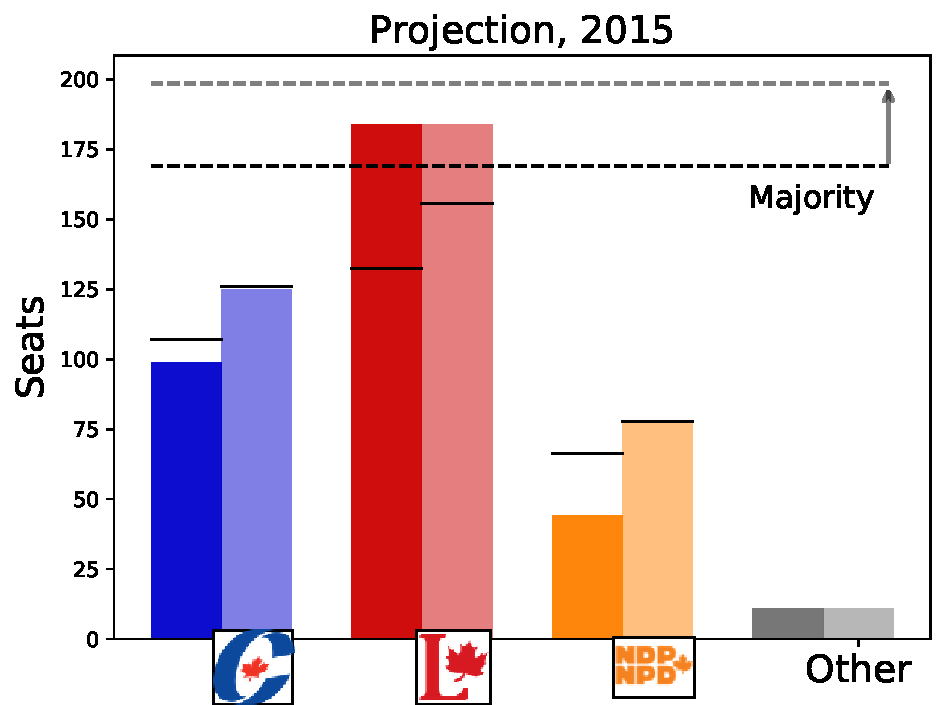
\includegraphics[width=0.50\textwidth,clip]{PR_calcs/data/raw_2015/PMM_out/PMM_projections}
  \caption{ Seat distribution following the 2015 federal election, using the same conventions as in Fig.~\ref{fig:projection_2019}.}
\label{fig:projection_2015}
\end{figure}



%----------------------------------------------------------------------------------------
%	Ceiling Parliament size
%----------------------------------------------------------------------------------------
\section{Extreme Split-Ballot Scenarios}

Data from recent elections indicate that PMM would be sufficient to establish a representative parliament with minimal expansion, however, we can imagine pathological cases.

Consider the extreme case where an under-represented party, $X$, receives zero \--or few\-- constituency seats, and yet is awarded nearly 100\% of the second-ballot votes.
Of course, this is exceedingly unlikely in practice, and would be even more implausible, given measures against decoy-lists (see conclusion, main text).
Nevertheless, for this hypothetical scenario a truly proportional legislature would require adding an \emph{infinite} number of supplemental MPs from party \textbf{$X$}.

To avoid this problem, a hard upper limit must be established \--for example, twice the number of constituencies. In our model, this quantity $\hat N \stackrel{!}{\le} N_{\textrm{max}} = 2 N$ is set as our upper-limit to ensure that constituent MPs are never in the minority, although more conservative constraints (i.e., smaller values of $N_{\textrm{max}}$) are also possible, and have been used in other MM systems.
The general rule remains:

\begin{align}
\label{eq:Nlimits}
N &\le& \hat{N} &\le& N_{\textrm{max}} \\
FPP &\le& PMM &\le& MM
\end{align}

The inequalities above serve to highlight that PMM will entail more seats than FPP, but fewer than traditional MM, as employed in, for example, Germany.
Both the upper and lower limits of this system (i.e., standard FPP and MM models) have been tested and shown practical in a functioning democracy. PMM seeks an optimal combination therein and is constrained to ensure that it can never go beyond the limits of what has been tested and shown to work.

% Finally, the 5\% threshold has been used as a filter of national support to limit supplementary seats to sincere and credible parties.
% The fact that this has the effect of encouraging parties to seek broad-based support throughout the country may be seen as a design feature, promoting national unity, however, it will likely be met with opposition be an established regional party such as the Bloc Quebecois.
% A palatable compromise may be to set the threshold at "5\% support nationally, \emph{or} 10\% support in at least one province...". In practice, the BQ has consistently exceeded this threshold, and the point may be moot.



\end{document}
